\section{Rendering Architecture}
The rendering system of our game is managed by a central \texttt{Renderer} class, which oversees all aspects of drawing the game's graphical elements using the Raylib library \cite{raylib}. This includes rendering the world, entities, the terrain, and the Heads-Up Display (HUD) as can be seen in fig. \ref{fig:new_game}.


  % \begin{figure}[h!]
  %   \centering
  %   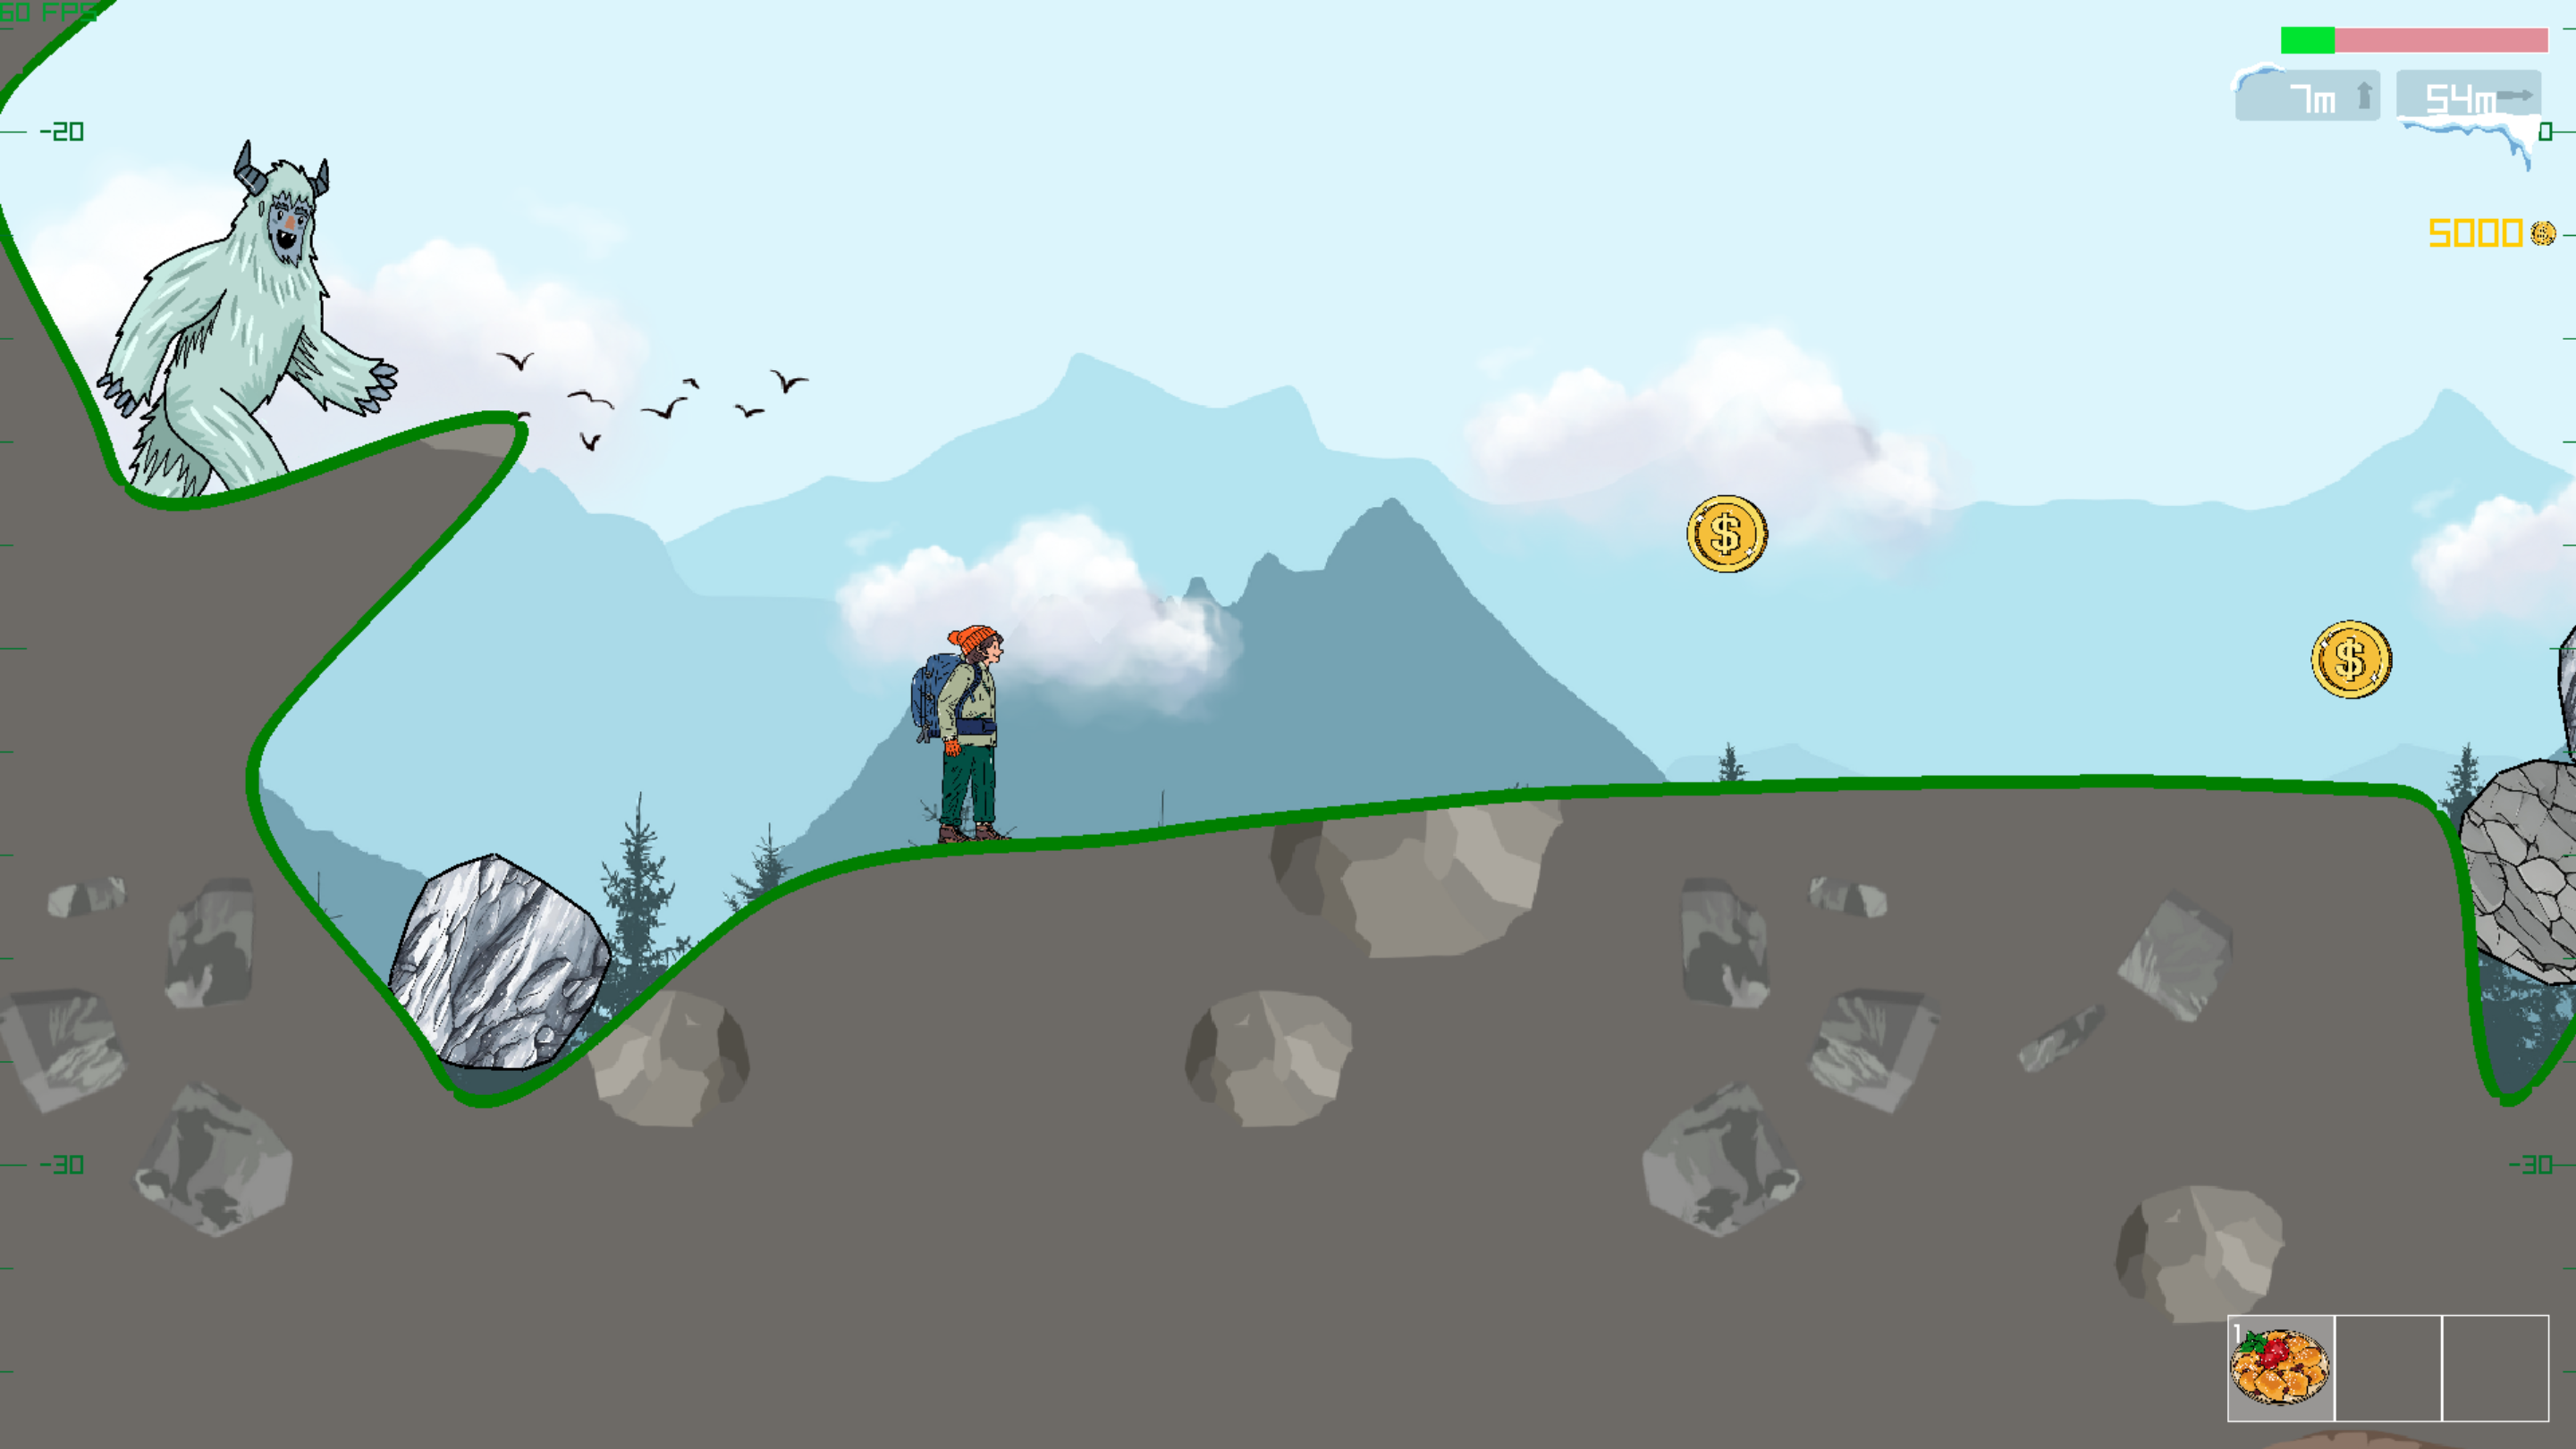
\includegraphics[width=0.45\textwidth]{figures/Ingame-Picture.png}
  %   \caption{In-game screenshot showing the rendering of entities, terrain, and HUD.}
  %   \label{fig:ingame}
  % \end{figure}

  \subsection{Main Renderer Class}

The \texttt{Renderer} class serves as the core component of the game's rendering pipeline. It is initialized with several key objects, including the world, camera, and resource manager, as well as sub-renderers like the \texttt{EntityRenderer}, \texttt{TerrainRenderer}, and \texttt{HudRenderer}. These sub-renderers handle rendering in a modular and efficient way, keeping different aspects of the world separate yet cohesive. The primary tasks of the \texttt{Renderer} include:

    \begin{itemize}
        \item Managing the camera view and adjusting its position based on the player's movements.
        \item Rendering the game's background dynamically.
        \item Delegating the rendering of entities, terrain, and HUD to the respective sub-renderers.
    \end{itemize}

  \subsubsection{Camera Initialization}

    The \texttt{Renderer} needs to initialize the camera. This camera setup is based on the dimensions of the world, ensuring that the entire world is visible on the screen with the correct zoom level:

    \begin{itemize}
        \item The world boundaries are determined using the game's unit-to-pixel ratio.
        \item The zoom level is calculated to fit the world width within the screen dimensions.
        \item The camera's position is centered within the visible portion of the world.
    \end{itemize}

    The camera is then updated dynamically during gameplay, adjusting to track the player's movements while maintaining smooth transitions.

  \subsubsection{Rendering Pipeline}

    The \texttt{draw()} method is responsible for the main rendering loop. It clears the screen and enters the 2D rendering mode with the camera applied.
    Then, the \texttt{Renderer} draws the background and calls the sub-renderers to draw the game's visual element.

  \subsubsection{Camera Effects and Fullscreen Support}

    In addition to basic rendering, the \texttt{Renderer} also handles visual effects such as camera shake, used to simulate rumble when certain events occur (e.g., a large rock falling nearby). The shake effect gradually dampens based on a visual constant and adds a layer of immersion to the gameplay experience.

    The \texttt{Renderer} also supports fullscreen mode, allowing players to choose between windowed and fullscreen display. 
    This feature is controlled through the game's configuration settings and cannot be adjusted at runtime, due to visual bugs occurring while toggling.

  \subsection{Sub-Renderers}

    The \texttt{Renderer} class delegates specific rendering tasks to various sub-renderers, each responsible for a distinct portion of the graphical output.

\subsubsection{TerrainRenderer}

The \texttt{TerrainRenderer} class is responsible for rendering the terrain, one of the primary visual components of the game.
The Renderer can convert the ground points into a series of 2D coordinates, which are then passed to the \texttt{poly2tri} library \cite{poly2tri} for triangulation.
This process creates a set of triangles that form the visual mesh of the mountain.
The generated triangles are stored as vertex data, which are used to draw the mountain with the texture applied.
It uses the triangulated mesh from the terrain data to apply a repeating texture to simulate a continuous mountainous background.
      This renderer loads and applies a repeating mountain texture, adjusting dynamically to camera view and terrain changes but updates only when necessary to minimize computational overhead.
      The rendering logic involves determining the visible terrain area, checking for boundary or vertex updates, and recalculating the mesh if needed. 
      The terrain is then rendered by applying the texture to the triangulated mesh.
To generate the mountain surface, the class relies on the terrain's polyline representation.

    \subsubsection{EntityRenderer}

      The \texttt{EntityRenderer} class is responsible for rendering dynamic game entities, such as the hiker, the monster, rocks, and in-game items. 
      It ensures each entity is drawn on the screen, manages animations, and provides debug capabilities for easier visualization of entity states. 
      The primary function of this class is to render entities using texture mapping and transformations. 
      Each entity’s attributes, such as position, size, rotation, and texture, are considered during rendering, allowing for accurate placement, scaling, and orientation on the screen.
This class also manages the Animation of entities.
Animation data, stored within each entity’s information, is used to update the current frame to be rendered of the animation according to the elapsed time.
      Certain entities, such as the hiker and rocks, have specialized rendering logic. 
      For example, the hiker is rendered differently depending on their movement state, including jumping, walking, or crouching. 
      Rocks can be rendered as textured polygons in their normal state, while destroyed rocks involve rendering explosions using an animation.
      
    \subsubsection{HudRenderer}

      The \texttt{HudRenderer} class renders essential HUD elements like the player's health, score, inventory, and altitude, providing real-time feedback during gameplay. It tracks the player's status and environment, updating accordingly.

    \subsection{Debug Mode}

The rendering system includes a debug mode that provides developers with additional visual information to aid in identifying rendering issues, verifying game state, and ensuring that the visual elements of the game are functioning as intended.
      It also removes unnecessary textures that would otherwise clutter the screen. 
      This mode can be toggled on and off, allowing for a clean and unobtrusive gameplay experience when not needed. 
      The debug mode includes the following features:

      \begin{itemize}
        \item \textbf{Entity Debugging:} Visualizes entity metadata like hitboxes or collection radii, making it easier to identify issues with entity positioning and interactions.
          \item \textbf{Terrain Debugging:} Renders the terrain's vertices and triangles, helping developers verify the correctness of the terrain mesh generation.
      \end{itemize}

      \vspace{-\abovedisplayskip}
      \begin{figure}[h!]
        \centering
        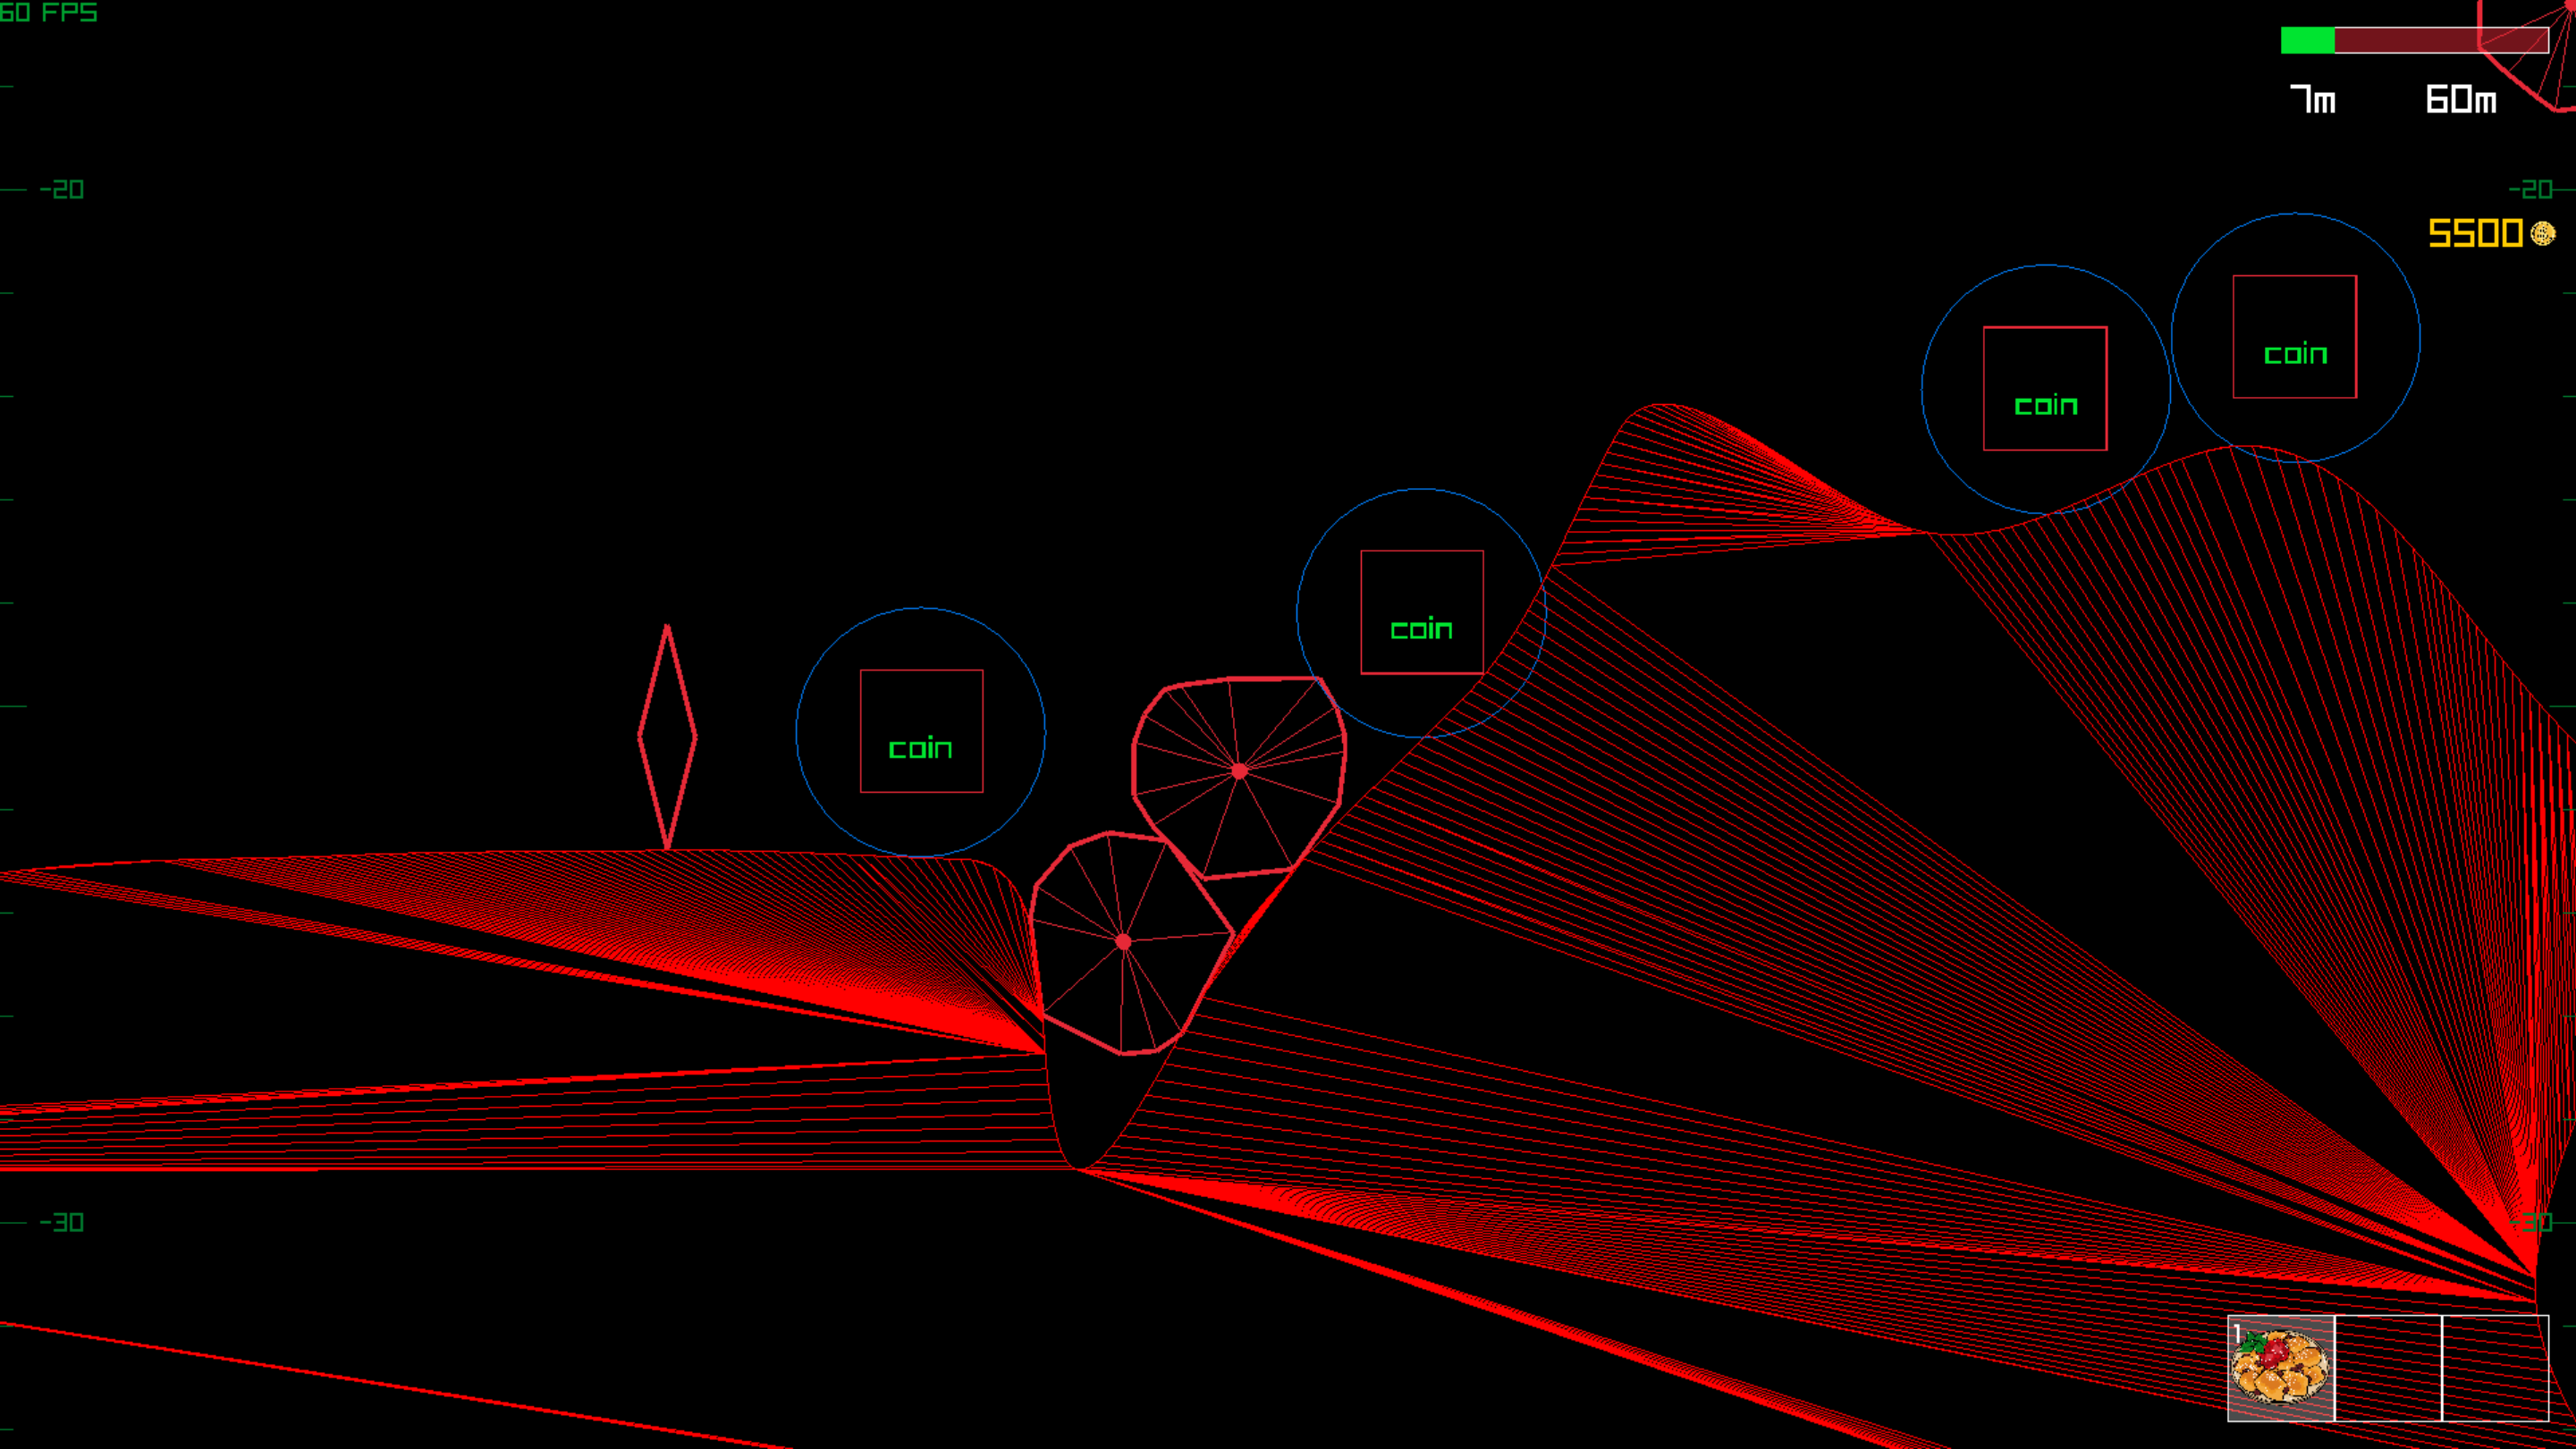
\includegraphics[width=0.45\textwidth]{figures/Debug-Mode.png}
        \caption{Debug mode visualization of hitboxes and terrain triangulation.}
        \label{fig:debug_mode}
      \end{figure}

      In fig. \ref{fig:debug_mode}, the debug mode visualization of the terrain triangulation is shown, as well as the hitboxes of the entities, 
      for example the hiker as a diamond shape, rocks as polygons with a centroid, and items as squares with a blue circle around them indicating the collection radius.
    
    \subsection{Optimizations}
      The renderer optimizes performance by only updating the terrain mesh when necessary, such as when boundaries shift or vertices change, avoiding unnecessary recalculations during each frame. 
      Additionally, animations are updated only when the time since the last frame exceeds the animation frame time, and entities that are destroyed and have completed their animations are removed from the rendering cycle. 
      